\section{Chapter 1 - Optimization Models}

\subsection{Tuesday 01/14/2025}
\subsubsection{Modeling Overview}
An optimization problem is represented by degrees of freedom that inform decisions. The degrees of freedom of a problem dictate the number of decisions that can be made.
\begin{itemize}
    \item n Decisions $> 0 \implies$ optimization problem
    \item n decisions $= 0 \implies$ simulation
\end{itemize}
The number of decisions is equal to the degrees of freedom, which is equivalent to the number of variables minus the number of inequalities.
\subsubsection{Example Problem}
This example problem will use a toy example of minimizing the perimeter of a rectangle with side lengths $x$ and $y$.

\begin{align}
  \text{minimize} & \quad P \\
  \text{subject to} & \quad xy = 2000 \\
  & \quad P = 2x + 2y \\
  & \quad x \geq 0, y \geq 0
\end{align}
with variables $x, y, P$. Since there are two equalities in the optimization problem above and three variables, there is one degree of freedom. This can be seen more plainly by reformulating the problem into the below problem
\begin{align}
    \text{minimize} & \quad 2 (\frac{2000}{y})+2y \\
    \text{subject to} & \quad y \geq 0
\end{align}
\subsubsection{General Optimization Definitions}
A general optimization problem can be written as
\begin{align}
  \text{minimize} & \quad F(x,y) \\
  \text{subject to} & \quad h(x,y) = 0 \\
  & \quad g(x,y) \leq 0
\end{align}
where $x \in \mathbb{R}^n, y \in \{ 0,1 \}^m$. This general optimization problem can be broken down into different problems with levels of complexity. \\ \\
Firstly, a \textbf{linear program} (LP) is defined as 
\begin{align}
  \text{minimize} & \quad F(x) \\
  \text{subject to} & \quad h(x) = 0 \\
  & \quad g(x) \leq 0
\end{align}
Where $x \in \mathbb{R}^n$ and $F,h,g$ are affine functions. Linear problems typically make many approximations about the real physics/constraints that are in the world. These approximations are a tradeoff with computational tractability. The Simplex method is typically used to solve linear programs. \\ \\
Secondly, a \textbf{non-linear program}  (NLP) is defined as  
\begin{align}
    \text{minimize} & \quad F(x) \\
    \text{subject to} & \quad h(x) = 0 \\
    & \quad g(x) \leq 0
\end{align}
Where $x \in \mathbb{R}^n$ and any of the functions $F,h,g$ are non-linear. A subset of NLPs are those problems that are \textit{convex}. Convexity in a non-linear program is achieved when $F,g$ are convex functions and $h$ is an affine function. Some algorithms that are used to solve NLPs are SQP, IPOPT. \\ \\
A higher degree of complexity, are \textbf{mixed integer linear programs} (MILP) defined as
\begin{align}
    \text{minimize} & \quad F(x,y) \\
    \text{subject to} & \quad h(x,y) = 0 \\
    & \quad g(x,y) \leq 0
\end{align}
where $x \in \mathbb{R}^n, y \in \{ 0,1 \}^m$. and $F,h,g$ are affine functions which can be represented as $F(x,y) = Ax + By$. These problems have applications in chemical engineering with examples such as biomass, waste, and fuel supply chains.  In a biomass biorefinery location problem, you would have a set of locations to pick from $y$ and you want to minimize the cost. An algorithm used to solve these problems is branch-and-bound. \\ \\
With the highest degree of complexity, a \textbf{mixed integer non-linear program} (MINLP) is defined as
\begin{align}
    \text{minimize} & \quad F(x,y) \\
    \text{subject to} & \quad h(x,y) = 0 \\
    & \quad g(x,y) \leq 0
\end{align}
where $x \in \mathbb{R}^n, y \in \{ 0,1 \}^m$ and any of the $F,h,g$ functions are non-linear. BARON, SCIP, MAINGO are algorithms that have been developed in the last 10 years in response to solve MINLPs. Chemical engineering is naturally non-linear and there has been a big push from the chemical optimization community to create solutions for MINLPs. These are complex problems but also important problems. \\ \\

\subsubsection{Specific Model Criteria}

Optimization problems can be also defined by the \textbf{number of objectives} they have.
\begin{itemize}
    \item Single objective
    \item Multiple objective
\end{itemize}
Multiple objectives introduce a tradeoff between different objectives with each other. If the number of objectives is low, then it is easy to identify and visualize the tradeoffs. The concept of pareto optimal will be explored further in the course.
\begin{align}
  \text{minimize} & \quad \langle F_1(x), F_2(x), \dots, F_k(x) \rangle
\end{align}
\\ \\
Optimization problems can also have a level of \textbf{uncertainty} in the problem. For example, the price and cost parameters may be random and uncertain. The majority of time, the randomness and uncertainty in models are ignored by modelers. A good guess is used and substituted for the random parameters such as an average or other estimate. However, it is possible to create stochastic models that attempt to handle uncertainty.
\begin{itemize}
    \item Deterministic models: Uncertainty is ignored and stochastic parameters are replaced by a fixed "good guess".
    \item Stochastic models: Uncertainty is handled and incorporated in the constraints.
\end{itemize}
Typically, stochastic models are significantly more difficult to compute than deterministic models. So, a deterministic model should be used and solved before a stochastic one is approached. \\ \\
Optimization models are also specified by their \textbf{type/number of constraints}
\begin{itemize}
    \item Unconstrained
    \item Constrained
\end{itemize}

\subsubsection{Optimization Concepts}
For general optimization problem defined above, a \textbf{feasible region} is defined as the set of $\langle x, y \rangle$ that satisfy all equalities and inequalities.

\begin{align}
  \text{minimize} & \quad -xy \\
  \text{subject to} & \quad x \geq 0, x \leq 1 \\
  & \quad y \geq 0, y \leq 1
\end{align}
For this problem, the feasible region $R$ is
\begin{equation}
    R(x,y) = \{ ( x, y ) | 0 \leq x \leq 1, 0 \leq y \leq 1  \}
\end{equation}

A \textbf{local minimum} with respect to a distance $\varepsilon$ is defined as a point $(x^*, y^*)$ that satisfies $ F(x^*, y^*) \leq F(x,y), \| x^* - x \| \leq \varepsilon$. A \textbf{global minimum} is a point that satisfies $ F(x^*, y^*) \leq F(x,y)$.

\begin{figure}[htbp]
  \centerline{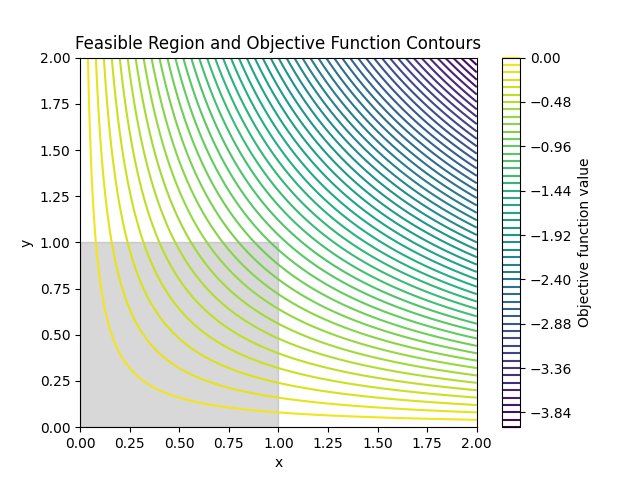
\includegraphics[width=0.50\textwidth]{chapters/01142025_feasible_region.png}}
  \caption{A plot of the optimization problem $F(x,y) = -xy$}
  \label{fig:01142025_feasible_region}
\end{figure}
